\def\year{2017}\relax
%File: formatting-instruction.tex
\documentclass[letterpaper]{article} %DO NOT CHANGE THIS
\usepackage{aaai18}  %Required
\usepackage{times}  %Required
\usepackage{helvet}  %Required
\usepackage{courier}  %Required
\usepackage{url}  %Required
\usepackage{graphicx}  %Required
\frenchspacing  %Required
\setlength{\pdfpagewidth}{8.5in}  %Required
\setlength{\pdfpageheight}{11in}  %Required
%PDF Info Is Required:
  \pdfinfo{}
\setcounter{secnumdepth}{0}

\usepackage{amsmath}
\usepackage{amssymb}
\usepackage{amsthm}
\usepackage{multirow}
\usepackage{tikz}
\usepackage{comment}

\usepackage{graphicx}
\usepackage{caption}
\usepackage{subcaption}
\usepackage{listings}
\usepackage{multicol}
\usepackage{arydshln}
\usetikzlibrary{calc,backgrounds,positioning,fit}


\newcommand{\tup}[1]{{\langle #1 \rangle}}

\newcommand{\pre}{\mathsf{pre}}     % precondition
\newcommand{\del}{\mathsf{del}}     % effect
\newcommand{\add}{\mathsf{add}}     % effect
\newcommand{\eff}{\mathsf{eff}}     % effect
\newcommand{\cond}{\mathsf{cond}}   % conditional effect
\newcommand{\true}{\mathsf{true}}   % true
\newcommand{\false}{\mathsf{false}} % false
\newcommand{\PE}{\mathrm{PE}}     % precondition
\newcommand{\strips}{\textsc{Strips}}     % precondition



\newtheorem{theorem}{Theorem}
\newtheorem{lemma}[theorem]{Lemma}
\newtheorem{definition}[theorem]{Definition}


\begin{document}

\title{Learning \strips\ action models with classical planning}

\author{Diego Aineto\and Sergio Jim\'enez\and Eva Onaindia\\
{\small Departamento de Sistemas Inform\'aticos y Computaci\'on}\\
{\small Universitat Polit\`ecnica de Val\`encia.}\\
{\small Camino de Vera s/n. 46022 Valencia, Spain}\\
{\small \{dieaigar,serjice,onaindia\}@dsic.upv.es}}

\maketitle
\begin{abstract}
This paper presents a novel approach for learning \strips action models from examples that compiles this particular inductive learning task into classical planning. Interestingly, the compilation approach is flexible to different amounts of available input knowledge; the learning examples can range from a set of plans (with their corresponding initial and final states) to just a set of initial and final states (no intermediate action or state is given). What is more, the compilation accepts partially specified action models and can be used to validate whether certain observations of plan executions follow a given \strips\ action model, even if this model is not fully specified.
\end{abstract}


\section{Introduction}
Besides {\em plan synthesis}~\cite{ghallab2004automated,geffner:book:2013}, planning action models are also useful for {\em plan/goal recognition}~\cite{ramirez2012plan}. At both planning tasks, an automated planner is required to reason about action models that correctly and completely capture the possible world transitions. Unfortunately, building planning action models is complex, even for planning experts, and this knowledge acquisition task is a bottleneck that limits the potential of automated planning~\cite{kambhampati:modellite:AAAI2007}.

On the other hand, Machine Learning (ML) has shown to be able to compute a wide range of different kinds of models from examples~\cite{michalski2013machine}. The application of inductive ML to the learning of \strips\ action models~\cite{fikes1971strips}, the vanilla action model for planning, is not straightforward though:
\begin{itemize}
\item The inputs to ML algorithms (the learning/training data) usually are finite vectors encoding the value of fixed features in a given set of objects. The input for learning planning action models are observations of plan executions (where each plan possibly has different length).
\item The traditional output of ML algorithms is a scalar value (an integer, in the case of {\em classification} tasks, or a real value, in the case of {\em regression} tasks). When learning \strips\ action models the output is, for each action, the sets of preconditions, negative and positive effects, that define the possible state transitions.
\end{itemize}

The learning of \strips\ action models is a well-studied problem with sophisticated algorithms, like {\sc ARMS}~\cite{yang2007learning}, {\sc SLAF}~\cite{amir:alearning:JAIR08} or {\sc LOCM}~\cite{cresswell2013acquiring} that do not require full knowledge of the intermediate states traversed by the example plans. Motivated by recent advances on the synthesis of different kinds of generative models with classical planning~\cite{bonet2009automatic,segovia2016hierarchical,segovia2017generating}, this paper introduces an innovative approach for learning \strips\ action models that can be defined as a classical planning compilation. The compilation approach is appealing because it opens the door to the bootstrapping of planning action models but also because:
\begin{enumerate}
\item Is flexible to different amounts of available input knowledge. The learning examples can range from a set of plans (with their corresponding initial and final states) to just a set of initial and final states where no intermediate state  or action is observed.
\item Accepts previous knowledge about the structure of the actions in the form of partially specified action models. In the extreme, the compilation could be used to validate whether observed plan executions are valid for a given \strips\ action model.
\end{enumerate}

The paper is organized as follows. The first section presents the classical planning model, its extension to conditional effects (which is a requirement of the proposed compilation) and formalizes the \strips\ action model (the output of the addressed learning task). The second section formalizes the learning of \strips\ action models with regard to different amounts of available input knowledge. The third and fourth sections describe our approach for addressing this particular learning task by compiling it into classical planning and how previous knowledge can be introduced in the compilation to constrain the space of possible action models and make learning more practicable. Finally, last sections report the data collected during the empirical evaluation of our approach, discuss the strengths and weaknesses of our approach and propose several opportunities for future research.


\section{Background}
This section defines the planning models used on this work and the output of the learning task addressed in the paper.

\subsection{Classical planning}
We use $F$ to denote the set of {\em fluents} (propositional variables) describing a state. A {\em literal} $l$ is a valuation of a fluent $f\in F$, i.e. either~$l=f$ or $l=\neg f$. A set of literals $L$ represents a partial assignment of values to fluents (WLOG we assume that $L$ does not assign conflicting values to any fluent). We use $\mathcal{L}(F)$ to denote the set of all literal sets on $F$, i.e.~all partial assignments of values to fluents.

A {\em state} $s$ is a total assignment of values to fluents, i.e. $|s|=|F|$, so the size of the state space is $2^{|F|}$. Explicitly including negative literals $\neg f$ in states simplifies subsequent definitions but often, we abuse notation by defining a state $s$ only in terms of the fluents that are true in $s$, as is common in \strips\ planning.

A {\em classical planning frame} is a tuple $\Phi=\tup{F,A}$, where $F$ is a set of fluents and $A$ is a set of actions. Each action $a\in A$ comprises three sets of literals:
\begin{itemize}
\item $\pre(a)$, called {\em preconditions}, that defines the literals that must hold for the action to be applicable.
\item $\eff^+(a)$, called {\em positive effects}, that defines the fluents set to true by the action application.
\item $\eff^-(a)$, called {\em negative effects}, that defines the fluents set to false by the application of the action. 
\end{itemize}
We say that an action $a\in A$ is {\em applicable} in state $s$ iff $\pre(a)\subseteq s$, and the result of applying $a$ in $s$ is the {\em successor state} $\theta(s,a)=\{s\setminus\eff^-(a))\cup\eff^+(a)\}$.

A {\em classical planning problem} is a tuple $P=\tup{F,A,I,G}$, where $I$ is an initial state and $G\in\mathcal{L}(F)$ is a goal condition. A {\em plan} for $P$ is an action sequence $\pi=\tup{a_1, \ldots, a_n}$ that induces a state sequence $\tup{s_0, s_1, \ldots, s_n}$ such that $s_0=I$ and, for each {\small $1\leq i\leq n$}, $a_i$ is applicable in $s_{i-1}$ and generates the successor state $s_i=\theta(s_{i-1},a_i)$. A plan $\pi$ {\em solves} $P$ iff $G\subseteq s_n$, i.e.~if the goal condition is satisfied at the last state reached after following the application of $\pi$ in $I$.


\subsection{Classical planning with conditional effects}
Our approach for leaning \strips\ action models is compiling this leaning task into a classical planning task with conditional effects. Conditional effects allow us to compactly define actions whose effects depend on the current state. Many classical planners cope with conditional effects without compiling them away. In fact, supporting conditional effects is a requirement of IPC-2014~\cite{vallati:IPC:AIM2015} and IPC-2018.

Now an action $a\in A$ has a set of literals $\pre(a)\in\mathcal{L}(F)$, called the {\em precondition}, and a set of {\em conditional effects} $\cond(a)$. Each conditional effect $C\rhd E\in\cond(a)$ is composed of two sets of literals $C\in\mathcal{L}(F)$, the {\em condition}, and $E\in\mathcal{L}(F)$, the {\em effect}.

An action $a\in A$ is {\em applicable} in state $s$ if and only if $\pre(a)\subseteq s$, and the resulting set of {\em triggered effects} is
\[
triggered(s,a)=\bigcup_{C\rhd E\in\cond(a),C\subseteq s} E,
\]
i.e.~effects whose conditions hold in $s$.

The result of applying action $a$ in a state $s$ is the {\em successor} state $\theta(s,a)=\{s\setminus\del(s,a))\cup\add(s,a)\}$ where $del(s,a)\subseteq triggered(s,a)$ and $add(s,a)\subseteq triggered(s,a)$ are the triggered negative and positive effects .


\subsection{The \strips\ action schema and the {\em variable} objects}
This work addresses the learning of PDDL action schemes that follow the \strips\ requirement~\cite{mcdermott1998pddl,fox2003pddl2}. Figure~\ref{fig:stack} shows the schema that corresponds to the {\em stack} action from a four-operator {\em blocksworld}~\cite{slaney2001blocks}.

\begin{figure}
\begin{scriptsize}
\begin{verbatim}
(:action stack
  :parameters (?x1 ?x2 - object)
  :precondition (and (holding ?x1) (clear ?x2))
  :effect (and (not (holding ?x1)) (not (clear ?x2))
               (handempty) (clear ?x1) (on ?x1 ?x2)))
\end{verbatim}
\end{scriptsize}
 \caption{\small Example of a \strips\ operator schema that corresponds to the {\em stack} action from the {\em blocksworld} represented in PDDL.}
\label{fig:stack}
\end{figure}

To formalize the output of the learning task, we assume that there exists a set of {\em predicates} $\Psi$ and that fluents $F$ are instantiated from these predicates, as in PDDL. Each predicate $p\in\Psi$ has an argument list of arity $ar(p)$. Given a set of objects $\Omega$, the set of fluents $F$ is then induced by assigning objects in $\Omega$ to the arguments of predicates in $\Psi$, i.e.~$F=\{p(\omega):p\in\Psi,\omega\in\Omega^{ar(p)}\}$ s.t. $\Omega^k$ is the $k$-th Cartesian power of $\Omega$. Likewise, we assume that actions $a\in A$ are instantiated from \strips\ operator schemes. 

Let $\Omega_v=\{v_i\}_{i=1}^{\operatorname*{max}_{a\in A} ar(a)}$ be a new set of objects, $\Omega\cap\Omega_v=\emptyset$, that represents {\em variable names} and that is bound by the maximum arity of an action in a given planning frame. For instance, in a three-block blocksworld $\Omega=\{block_1, block_2, block_3\}$ while $\Omega_v=\{v_1, v_2\}$ because the operators with the maximum arity, {\small\tt stack} and {\small\tt unstack}, have two parameters each.

Let us define also a new set of fluents $F_{v}$, s.t. $F\cap F_v=\emptyset$, that results instantiating $\Psi$ using only {\em variable objects} in $\Omega_v$. This set defines the elements that can appear in an action schema. In the blocksworld $F_v$={\small\tt\{handempty, holding($v_1$), holding($v_2$), clear($v_1$), clear($v_2$), ontable($v_1$), ontable($v_2$), on($v_1,v_1$),on($v_1,v_2$), on($v_2,v_1$),on($v_2,v_2$)\}}. 

We are now ready to define $\Xi$, a set of operator schema $\xi=\tup{head(\xi),pre(\xi),add(\xi),del(\xi)}$ such that:
\begin{itemize}
\item $head(\xi)=\tup{name(\xi),pars(\xi)}$, is the operator {\em header} defined by its name and $pars(\xi)=\{v_i\}_{i=1}^{ar(\xi)}$, an enumeration of the variable objects bound by the operator arity. The headers for a 4-operator blocksworld are: {\small\tt pickup($v_1$), putdown($v_1$), stack($v_1,v_2$)} and {\small\tt unstack($v_1,v_2$)}.
\item The preconditions $pre(\xi)\subseteq F_v$, the negative effects $del(\xi)\subseteq F_v$, and the positive effects $add(\xi)\subseteq F_v$ such that, $del(\xi)\subseteq pre(\xi)$, $del(\xi)\cap add(\xi)=\emptyset$ and $pre(\xi)\cap add(\xi)=\emptyset$.
\end{itemize}


\section{Learning \strips\ action models}
Learning \strips\ action models from fully available input knowledge, i.e. from plans where the {\em pre-} and {\em post-states} of every action in a plan are available, is straightforward. In this case, because intermediate states are available, \strips\ operator schemes are derived lifting the literals that change between the pre and post-state of the corresponding action executions. Preconditions are derived lifting the minimal set of literals that appears in all the pre-states that correspond to the same operator schema.

This section formalizes more challenging learning tasks, where less input knowledge is available.

\subsection{Learning from (initial, final) state pairs}
This learning task corresponds to observing an agent acting in the world but watching only the results of its plan executions. No information about the actions in the plans is given however, we assume that the headers of the operators schema are known.

This learning task is formalized as $\Lambda=\tup{\Psi,\Sigma}$:
\begin{itemize}
\item $\Psi$, the set of predicates that define the abstract state space of a given planning domain.
\item $\Sigma=\{\sigma_1,\ldots,\sigma_{\tau}\}$, a set of (initial, final) state pairs s.t., for every {\tt\small $1\leq t\leq \tau$}, a pair $\sigma_t=(s_0^t,s_{n}^t)$ comprises the {\em final} state $s_{n}^t$ resulting from executing an unknown plan $\pi_t$ starting from a given {\em initial} state $s_0^t$.
\end{itemize}

A solution to the learning task $\Lambda$  is a set of operator schema $\Xi$ that is compliant with the predicates in $\Psi$, and the given set of initial and final states $\Sigma$.

In this learning scenario, a solution must not only determine a possible \strips\ action model but also the plans $\pi_t$ that explain the given states $\Sigma$ using the learned \strips\ model.

\subsection{Learning from labeled plans}
Here we augment the amount of provided input knowledge and define the learning task as $\Lambda'=\tup{\Psi,\Sigma,\Pi}$.

Now $\Pi=\{\pi_1,\ldots,\pi_{\tau}\}$ is a given set of example plans where each plan $\pi_t=\tup{a_1^t, \ldots, a_n^t}$, {\small $1\leq t\leq \tau$}, is an action sequence that induces the corresponding state sequence $\tup{s_0^t, s_1^t, \ldots, s_n^t}$ such that, for each {\small $1\leq i\leq n$}, $a_i^t$ is applicable in the state $s_{i-1}^t$ and generates the successor state $s_i^t=\theta(s_{i-1}^t,a_i^t)$.

A solution to a learning task $\Lambda'$ is a set of \strips\ operator schema $\Xi$ (with one schema $\xi=\tup{head(\xi),pre(\xi),add(\xi),del(\xi)}$ for each action with a different name in the example plans $\Pi$) that is compliant with the predicates in $\Psi$, the example plans $\Pi$, and their corresponding labels $\Sigma$. 

Figure~\ref{fig:lexample} shows an example of a learning task $\Lambda'$ in the blocksworld (the figure shows the content of $\Psi$, $\Pi$ and $\Sigma$). This learning task has a single learning example, $\Pi=\{\pi_1\}$ and $\Sigma=\{\sigma_1\}$, that corresponds to observing the execution of a plan for inverting a four-block tower.

\begin{figure}
{\tt ;;; Predicates in $\Psi$}
\begin{footnotesize}
\begin{verbatim}
(handempty) (holding ?o  - object)
(clear ?o - object) (ontable ?o - object)
(on ?o1 - object ?o2 - object)
\end{verbatim}
\end{footnotesize}

\vspace{0.2cm}

\begin{subfigure}{.25\textwidth}
{\tt ;;; Plan $\pi_1$}
\begin{footnotesize}
\begin{verbatim}
0: (unstack A B)
1: (putdown A)
2: (unstack B C)
3: (stack B A)
4: (unstack C D)
5: (stack C B)
6: (pickup D)
7: (stack D C)
\end{verbatim}
\end{footnotesize}
\end{subfigure}%
\begin{subfigure}{.6\textwidth}
{\tt ;;; Label $\sigma_1=(s_0^1,s_{n}^1)$}
\begin{lstlisting}[mathescape]
\end{lstlisting}
\vspace{0.1cm}
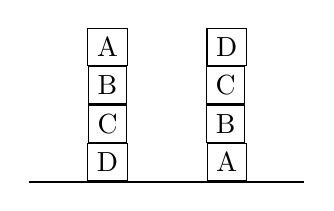
\begin{tikzpicture}[node distance = 0mm, block/.style args = {#1,#2}{fill=#1,text width=#2,shape=square}]
\node (initD) [draw]{D};
\node (initC) [draw, above=of initD.north]{C};
\node (initB) [draw, above=of initC.north]{B};
\node (initA) [draw, above=of initB.north]{A};
\draw[thick] (-1,-0.25) -- (2.5,-0.25);

\node (goalA) [draw, right=10mm of initD]{A};
\node (goalB) [draw, right=10mm of initC]{B};
\node (goalC) [draw, right=10mm of initB]{C};
\node (goalD) [draw, right=10mm of initA]{D};
\end{tikzpicture}
\vspace{0.6cm}
\end{subfigure}%

 \caption{\small Example of a task for learning a \strips\ action model in the blocksworld.}
\label{fig:lexample}
\end{figure}


\section{Learning \strips\ action models with planning}
Our approach for addressing a learning task $\Lambda$ or $\Lambda'$, is compiling it into a classical planning task with conditional effects. The intuition behind these compilations is that a solution to the resulting classical planning task is a sequence of actions that:
\begin{enumerate}
\item Programs the \strips\ action model $\Xi$. For each $\xi\in\Xi$, the solution plan has a prefix that determines the literals that belong to its $pre(\xi)$, $del(\xi)$ and $add(\xi)$ sets.
\item Validates the programmed \strips\ action model $\Xi$ using the given input knowledge (the set of labels $\Sigma$, and $\Pi$ if available).  For every label $\sigma_t\in \Sigma$, then $\Xi$ is used to produce a final state $s_{n}^t$ starting from the corresponding initial state $s_0^t$. We call this process the validation of the programmed \strips\ action model $\Xi$, at the learning example {\small $1\leq t\leq \tau$}. If information about the corresponding plan $\pi_t\in \Pi$ is available, then it is also used in the validation.
\end{enumerate}

To formalize our compilations we first define {\small $1\leq t\leq \tau$} classical planning instances $P_t=\tup{F,\emptyset,I_t,G_t}$ that belong to the same planning frame (i.e. same fluents and actions and differ only in the initial state and goals). The fluents $F$ are built instantiating the predicates in $\Psi$ with the objects appearing in the inputs. Formally $\Omega=\{o|o\in \bigcup_{\small 1\leq t\leq \tau} obj(s_0^t)\}$, where $obj$ is a function that returns the set of objects that appear in a fully specified state. The set of actions, $A=\emptyset$, is empty because the action model is initially unknown. Finally, the initial state $I_t$ is given by the state $s_0^t\in \sigma_t$ while goals $G_t$, are defined by the state $s_n^t\in \sigma_t$.

Now we are ready to formalize the compilations. We start with $\Lambda$, because this learning task requires fewer input knowledge. Given a learning task $\Lambda=\tup{\Psi,\Sigma}$ the compilation outputs a classical planning task $P_{\Lambda}=\tup{F_{\Lambda},A_{\Lambda},I_{\Lambda},G_{\Lambda}}$ such that:
\begin{itemize}
\item $F_{\Lambda}$ extends $F$ with:
\begin{itemize}
\item Fluents representing the programmed action model $pre_f(\xi)$, $del_f(\xi)$ and $add_f(\xi)$, for every $f\in F_v$ and $\xi \in \Xi$. If a fluent $pre_f(\xi)/del_f(\xi)/add_f(\xi)$ holds, it means that $f$ is a precondition/negative effect/positive effect in the \strips\ operator schema $\xi\in \Xi$. For instance in the working example the preconditions of the $stack$ schema are reprenseted by the fluents {\small\tt pre\_holding\_stack\_$v_1$} and {\small\tt pre\_clear\_stack\_$v_2$} set to true. 
\item A fluent $mode_{prog}$ indicating whether the operator schemes are being programmed or they are being validated (already programmed).
\item Fluents $\{test_t\}_{1\leq t\leq \tau}$, indicating the learning example where the programmed action model is being validated.
\end{itemize}
\item $I_{\Lambda}$, contains the fluents from $F$ that encode $s_0^1$ (the initial state of the first learning example), every $pre_f(\xi)\in F_{\Lambda}$ (our compilation assumes that initially any operator schema is programmed with every possible precondition, no negative effect and no positive effect) and $mode_{prog}$ set to true.
\item $G_{\Lambda}=\bigcup_{1\leq t\leq \tau}\{test_t\}$, indicates that the programmed action model is validated in all the learning examples.
\item $A_{\Lambda}$ contains actions of three different kinds:
\begin{enumerate}
\item The actions for programming an operator schema $\xi\in\Xi$, which includes:
\begin{itemize}
\item The actions for {\bf removing} a {\em precondition} $f\in F_v$ from the action schema $\xi\in\Xi$.

\begin{small}
\begin{align*}
\hspace*{7pt}\pre(\mathsf{programPre_{f,\xi}})=&\{\neg del_{f}(\xi),\neg add_{f}(\xi),\\
& pre_{f}(\xi), mode_{prog}\},\\
\cond(\mathsf{programPre_{f,\xi}})=&\{\emptyset\}\rhd\{\neg pre_{f}(\xi)\}.
\end{align*}
\end{small}

\item The actions for {\bf adding} a {\em negative} or a {\em positive} effect $f\in F_v$ to the action schema $\xi\in\Xi$.

\begin{small}
\begin{align*}
\hspace*{7pt}\pre(\mathsf{programEff_{f,\xi}})=&\{\neg del_{f}(\xi),\neg add_{f}(\xi),\\
& mode_{prog}\},\\
\cond(\mathsf{programEff_{f,\xi}})=&\{pre_{f}(\xi)\}\rhd\{del_{f}(\xi)\},\\
&\{\neg pre_{f}(\xi)\}\rhd\{add_{f}(\xi)\}.
\end{align*}
\end{small}
\end{itemize}

\item The actions for applying an already programmed operator schema $\xi\in\Xi$ bound with the objects $\omega\subseteq\Omega^{ar(\xi)}$. The binding of the operator schema is done implicitly by order of appearance of the action parameters, i.e. the variables in $pars(\xi)$ are bound to the objects in $\omega$ appearing at the same position. Figure~\ref{fig:compilation} shows the PDDL encoding of the action for applying a programmed operator $stack$.
\begin{small}
\begin{align*}
\hspace*{7pt}\pre(\mathsf{apply_{\xi,\omega}})=&\{pre_{f}(\xi)\implies p(\omega)\}_{\forall p\in\Psi,f=p(pars(\xi))},\\
\cond(\mathsf{apply_{\xi,\omega}})=&\{del_{f}(\xi)\}\rhd\{\neg p(\omega)\}_{\forall p\in\Psi,f=p(pars(\xi))},\\
&\{add_{f}(\xi)\}\rhd\{p(\omega)\}_{\forall p\in\Psi,f=p(pars(\xi))},\\
&\{mode_{prog}\}\rhd\{\neg mode_{prog}\}.
\end{align*}
\end{small}

\item The actions for updating the learning example {\tt\small $1\leq t\leq \tau$} where the programmed action model is validated.
\begin{small}
\begin{align*}
\hspace*{7pt}\pre(\mathsf{validate_{t}})=&G_t\cup\{test_j\}_{j\in 1\leq j<t}\cup\\
&\cup\{\neg test_j\}_{j\in t\leq j\leq \tau}\cup \{\neg mode_{prog}\},\\
\cond(\mathsf{validate_{t}})=&\{\emptyset\}\rhd\{test_t\}.
\end{align*}
\end{small}
\end{enumerate}
\end{itemize}


\begin{figure}[hbt]
\begin{scriptsize}
\begin{verbatim}
(:action apply_stack
  :parameters (?o1 - object ?o2 - object)
  :precondition
   (and (or (not (pre_on_stack_v1_v1)) (on ?o1 ?o1))
        (or (not (pre_on_stack_v1_v2)) (on ?o1 ?o2))
        (or (not (pre_on_stack_v2_v1)) (on ?o2 ?o1))
        (or (not (pre_on_stack_v2_v2)) (on ?o2 ?o2))
        (or (not (pre_ontable_stack_v1)) (ontable ?o1))
        (or (not (pre_ontable_stack_v2)) (ontable ?o2))
        (or (not (pre_clear_stack_v1)) (clear ?o1))
        (or (not (pre_clear_stack_v2)) (clear ?o2))
        (or (not (pre_holding_stack_v1)) (holding ?o1))
        (or (not (pre_holding_stack_v2)) (holding ?o2))
        (or (not (pre_handempty_stack)) (handempty)))
  :effect
   (and (when (del_on_stack_v1_v1) (not (on ?o1 ?o1)))
        (when (del_on_stack_v1_v2) (not (on ?o1 ?o2)))
        (when (del_on_stack_v2_v1) (not (on ?o2 ?o1)))
        (when (del_on_stack_v2_v2) (not (on ?o2 ?o2)))
        (when (del_ontable_stack_v1) (not (ontable ?o1)))
        (when (del_ontable_stack_v2) (not (ontable ?o2)))
        (when (del_clear_stack_v1) (not (clear ?o1)))
        (when (del_clear_stack_v2) (not (clear ?o2)))
        (when (del_holding_stack_v1) (not (holding ?o1)))
        (when (del_holding_stack_v2) (not (holding ?o2)))
        (when (del_handempty_stack) (not (handempty)))
        (when (add_on_stack_v1_v1) (on ?o1 ?o1))
        (when (add_on_stack_v1_v2) (on ?o1 ?o2))
        (when (add_on_stack_v2_v1) (on ?o2 ?o1))
        (when (add_on_stack_v2_v2) (on ?o2 ?o2))
        (when (add_ontable_stack_v1) (ontable ?o1))
        (when (add_ontable_stack_v2) (ontable ?o2))
        (when (add_clear_stack_v1) (clear ?o1))
        (when (add_clear_stack_v2) (clear ?o2))
        (when (add_holding_stack_v1) (holding ?o1))
        (when (add_holding_stack_v2) (holding ?o2))
        (when (add_handempty_stack) (handempty))
        (when (modeProg) (not (modeProg)))))
\end{verbatim}
\end{scriptsize}
 \caption{\small Action for applying an already programmed operator schema $stack$ as encoded in PDDL.}
\label{fig:compilation}
\end{figure}


\begin{lemma}
Any classical plan $\pi$ that solves $P_{\Lambda}$ induces an action model $\Xi$ that solves the learning task $\Lambda$.
\end{lemma}

\begin{proof}[Proof sketch]
\begin{small}
The compilation forces that once the preconditions of an operator schema $\xi \in \Xi$ are programmed, they cannot be altered. The same happens with the positive and negative effects that define an operator schema $\xi \in \Xi$ (besides they can only be programmed after the preconditions are programmed). Furthermore, once operator schemes are programmed they can only be applied because of the $mode_{prog}$ fluent. To solve $P_{\Lambda}$, there is only one way of achieving goals $\{test_t\}$, {\small $1\leq t\leq \tau$}: executing an applicable sequence of programmed operator schemes that reaches the final state $s_n^t$ defined in $\sigma_t$, starting from $s_0^t$ (defined in this same label). If this is achieved for all the input examples {\small $1\leq t\leq \tau$} of the learning task, it means that the programmed action model $\Xi$ is compliant with the provided input knowledge and hence, it is a solution to $\Lambda$.
\end{small}
\end{proof}

The compilation is {\em complete} in the sense that it does not discard any possible \strips\ action model.


Figure~\ref{fig:plan} shows a classical plan for solving a learning task of the $\Lambda$ kind. This classical plan programs and validates the operator schema {\tt\small stack} from the blocksworld (previously specified operator schemes for $pickup$, $putdown$ and $unstack$ are given), using the plan $\pi_1$ and label $\sigma_1$ shown in Figure~\ref{fig:lexample}. The plan steps $[0,8]$ are the actions for programming the preconditions of the {\tt\small stack} operator, steps $[9,13]$ are the actions for programming the operator effects and steps $[14,22]$ are actions for validating the programmed operators. The details of the compilation are explained in the remaining of the section.

\begin{figure}
\begin{small}
\begin{verbatim}
     0 : (program_pre_clear_stack_v1)
     1 : (program_pre_handempty_stack)
     2 : (program_pre_holding_stack_v2)
     3 : (program_pre_on_stack_v1_v1)
     4 : (program_pre_on_stack_v1_v2)
     5 : (program_pre_on_stack_v2_v1)
     6 : (program_pre_on_stack_v2_v2)
     7 : (program_pre_ontable_stack_v1)
     8 : (program_pre_ontable_stack_v2)
     9 : (program_eff_clear_stack_v1)
    10 : (program_eff_clear_stack_v2)
    11 : (program_eff_handempty_stack)
    12 : (program_eff_holding_stack_v1)
    13 : (program_eff_on_stack_v1_v2)
    14 : (apply_unstack a b i1 i2)
    15 : (apply_putdown a i2 i3)
    16 : (apply_unstack b c i3 i4)
    17 : (apply_stack b a i4 i5)
    18 : (apply_unstack c d i5 i6)
    19 : (apply_stack c b i6 i7)
    20 : (apply_pickup d i7 i8)
    21 : (apply_stack d c i8 i9)
    22 : (validate_1)
\end{verbatim}
\end{small}
 \caption{\small Example of a plan for programming and validating the operator schema $stack$ using the plan $\pi_1$ and label $\sigma_1$ shown in Figure~\ref{fig:lexample} as well as previously specified operator schemes for $pickup$, $putdown$ and $unstack$.}
\label{fig:plan}
\end{figure}


\section{Constraining the learning hypothesis space with additional input knowledge}
Here we show that further input knowledge can be used to constrain the space of the possible action models and make the learning of \strips action models more practicable.

\subsection{Example plans}
Here  we extend our compilation to address the learning scenario where, a set of plans is available. Given a learning task $\Lambda=\tup{\Psi,\Pi,\Sigma}$, the compilation outputs a classical planning task $P_{\Lambda}=\tup{F_{\Lambda},A_{\Lambda},I_{\Lambda},G_{\Lambda}}$ that extends $P_{\Lambda}'$ as follows:
\begin{itemize}
\item $F_{\Lambda}$ extends $F_{\Lambda'}$ with $F_{\Pi}=\{plan(name(\xi),\Omega^{ar(\xi)},j)\}$, the fluents to code the $j$ steps of plans in $\Pi$, where $F_{\pi_t}\subseteq F_{\Pi}$ encodes $\pi_t\in \Pi$. Fluents $at_j$ and $next_{j,j_2}$, {\small $1\leq j<j2\leq n$}, are also added to represent the current and next plan steps.
\item $I_{\Lambda}$ is extended with the fluents from $F_{\Pi}$ that encode the plan $\pi_1\in \Pi$, the fluents $at_1$ and $\{next_{j,j_2}\}$, {\small $1\leq j<j2\leq n$}, for indicating where to start validating the programmed action model. Goals are the same as in the previous compilation $G_{\Lambda}=G_{\Lambda}'=\bigcup_{1\leq t\leq \tau}\{test_t\}$.
\item With respect to $A_{\Lambda}$.
\begin{enumerate}
\item The actions for programming the preconditions/effects of a given operator schema $\xi\in\Xi$ are the same.
\item The actions for applying an already programmed operator have an extra precondition $f\in F_{\Pi}$, that encodes the current plan step, and extra conditional effects $\{at_{j}\}\rhd\{\neg at_{j},at_{j+1}\}_{\forall j\in [1,n]}$ for advancing to the next plan step. This mechanism forces that these actions are only applied as in the example plans.
\item The actions for updating the active test have an extra precondition, $at_{|\pi_t|}$, to indicate that the current plan $\pi_t$ was fully executed and extra conditional effects to load the next plan $\pi_{t+1}$:
\begin{small}
\begin{align*}
&\{f\}\rhd\{\neg f\}_{f\in F_{\pi_t}}, \{\emptyset\}\rhd\{f\}_{f\in F_{\pi_t+1}},\{\emptyset\}\rhd\{\neg at_{|\pi_t|},at_1\}.
\end{align*}
\end{small}
\end{enumerate}
\end{itemize}

\subsection{Previously specified action models}
Our compilation does not require to start learning \strips action models from scratch and accepts partially specified operator schema where some preconditions and effects are a priori known.

The known preconditions and effects are encoded as fluents $pre_f(\xi)$, $del_f(\xi)$ and $add_f(\xi)$ that are part of the initial state $I_{\Lambda'}$. The corresponding programming actions ($\mathsf{programPre_{f,\xi}}$ and $\mathsf{programEff_{f,\xi}}$) become unnecessary and are removed from $A_{\Lambda'}$ making the classical planning task $P_{\Lambda'}$ easier to be solved. To illustrate this, the classical plan of Figure~\ref{fig:plan} is a solution to a learning task for getting the blocksworld action model where the schemes for {\tt\small pickup}, {\tt\small putdown} and {\tt\small unstack} are known in advance.

In the extreme, when a fully specified \strips action model is given, the compilation validates whether an observed plan follows the given model. In this case, if a solution plan is found to $P_{\Lambda'}$, it means that the given \strips action model is {\em valid} for the given set of examples. If $P_{\Lambda'}$ is unsolvable it means that the given \strips action model is invalid since it is not compliant with all the given examples. Tools for plan validation like VAL~\cite{howey2004val} could also be used at this point.

\subsection{Static predicates}
A {\em static predicate} $p \in \Psi$ is a predicate that does not appear in the effects of any action schema~\cite{fox:TIM:JAIR1998}. Therefore, one can get rid of the mechanism for programming static predicates as action effects keeping the compilation complete. Formally, given a static predicate $p$:
\begin{itemize}
\item Fluents $del_f(\xi)$ and $add_f(\xi)$, such that $f\in F_v$ is an instantiation of the static predicate $p$ in the set of {\em variable} objects $\Omega_v$, can be discarded for every $\xi\in\Xi$.
\item Actions $\mathsf{programEff_{f,\xi}}$ (s.t. $f\in F_v$ is an instantiation of $p$ in $\Omega_v$) can also be discarded for every $\xi\in\Xi$.
\end{itemize}

Static predicates can also be used to constrain the space of possible preconditions by looking at the given labels. If a precondition $f\in F_v$ (s.t. $f\in F_v$ is an instantiation of a static predicate in $\Omega_v$) is not possible according to $\Sigma$, then the fluents $pre_f(\xi)$ and actions $\mathsf{programPre_{f,\xi}}$ can be discarded for every $\xi\in\Xi$. For instance in the {\em zenotravel} domain fluents $pre\_next\_board\_v1\_v1$, $pre\_next\_debark\_v1\_v1$, $pre\_next\_fly\_v1\_v1$, $pre\_next\_zoom\_v1\_v1$, $pre\_next\_refuel\_v1\_v1$ can be discarded (as well as their corresponding programming actions) because a precondition {\tt\small(next ?v1 ?v1 - flevel)} cannot be compliant with any state in $\Sigma$.

Likewise, static predicates can constrain the space of possible preconditions looking at the given example plans. In this case, fluents $pre_f(\xi)$ and actions $\mathsf{programPre_{f,\xi}}$ are discarded for every $\xi\in\Xi$ if a precondition $f\in F_v$ (s.t. $f\in F_v$ is an instantiation of a static predicate in $\Omega_v$) is not possible according to $\Pi$. Back to the {\em zenotravel} domain, if a example plan $\pi_t\in \Pi$ contains the action {\tt\small (fly plane1 city2 city0 fl3 fl2)} and the corresponding label $\sigma_t\in\Sigma$ contains the static fluent {\tt\small (next fl2 fl3)} but it does not include {\tt\small (next fl2 fl2)}, {\tt\small (next fl3 fl3)} or {\tt\small (next fl3 fl2)} it means that the only possible precondition including the static predicate is $pre\_next\_fly\_v1\_v2$.

In the evaluation of our approach we do not assume that the set of static predicates is given but compute a set of candidates of static predicates from the input examples to the learning task.


\section{Evaluation}
We evaluated our approach for learning STRIPS action models from different amounts of available input knowledge.

\subsection{Experimental setup}
All the experiments run on an Intel Core i5 3.10 GHz x 4 with 4 GB of RAM. The domains used in the evaluation are IPC domains that satisfy the STRIPS requirement~\cite{fox2003pddl2}, and are taken from the {\sc planning.domains} repository~\cite{muise2016planning}.

\subsubsection{The classical planner.}
The classical planner used to solve the instances that result from our compilations is the SAT-based classical planner {\sc Madagascar}~\cite{rintanen2014madagascar}. We decided to use a SAT-based planner because its ability to deal with planning instances populated with dead-ends. In addition, in a SAT-based classical planner all the actions for programming the STRIPS actions preconditions can be done in parallel, in a single planning step, because they do not interact reducing significantly the planning horizon. Likewise, all the actions for programming an action effect can also be applied in a single planning step.


\subsubsection{The evaluation metrics.}
The quality of the learned models is quantified with the {\em precision} and {\em recall} metrics. These two metrics are frequently used in pattern recognition, information retrieval and binary classification and are more informative that simply counting the number of model errors or computing the {\em symmetric difference} between the learned model and the baseline ~\cite{davis2006relationship}.

Intuitively precision gives a notion of {\em soundness} while recall gives a notion of the {\em completeness} of the learned models. Formally $Precision=\frac{tp}{tp+fp}$, where $tp$ is the number of true positives (predicates that correctly appear in the action model) and $fp$ is the number of false positives (predicates appear in the learned action model that should not appear). On the other hand recall is formally defined as $Recall=\frac{tp}{tp+fn}$ where $fn$ is the number of false negatives (predicates that should appear in the learned action model but are missing).


\subsubsection{The learning examples.}


\subsection{Learning action models from example plans}
Here we assess the performance of our learning approach when addressing $\Lambda$ learning tasks. Here the {\em precision} and {\em recall} metrics are computed in the learned models with respect to the actual models taken as reference. Table~\ref{tab:results_plans} summarizes the obtained results, precision ({\bf P}) and recall ({\bf R}) is computed separately for the preconditions ({\bf Pre}), positive effects ({\bf Add}) and negative Effects ({\bf Del}).

\begin{table}[hbt!]
	\begin{center}
		\resizebox{\columnwidth}{!}{%
		\begin{tabular}{l|l|l|l|l|l|l|l|l|}
			 & \multicolumn{2}{|c|}{\bf Pre} & \multicolumn{2}{|c|}{\bf Add} & \multicolumn{2}{|c|}{\bf Del} & \multicolumn{2}{|c|}{\bf All}\\ \cline{2-9}			
			  & \multicolumn{1}{|c|}{\bf P} & \multicolumn{1}{|c|}{\bf R} & \multicolumn{1}{|c|}{\bf P} & \multicolumn{1}{|c|}{\bf R} & \multicolumn{1}{|c|}{\bf P} & \multicolumn{1}{|c|}{\bf R} &  \multicolumn{1}{|c|}{\bf P} & \multicolumn{1}{|c|}{\bf R} \\
			\hline
			Blocks & 1.0 & 1.0 & 1.0 & 1.0 & 1.0 & 1.0 & 1.0 & 1.0 \\
			Driverlog & 1.0 & 0.43 & 0.67 & 0.86 & 1.0 & 0.86 & 0.89 & 0.71 \\
			Ferry & 0.80 & 0.57 & 1.0 & 1.0 & 1.0 & 1.0 & 0.93 & 0.86 \\
			Floortile & 0.54 & 0.64 & 0.90 & 0.82 & 1.0 & 0.91 & 0.81 & 0.79 \\
			Gripper & 1.0 & 0.67 & 1.0 & 1.0 & 1.0 & 1.0 & 1.0 & 0.89 \\
			Miconic & 0.75 & 0.33 & 1.0 & 0.75 & 0.75 & 1.0 & 0.83 & 0.69 \\
			Satellite & 0.67 & 0.29 & 1.0 & 1.0 & 1.0 & 0.75 & 0.89 & 0.68 \\
			Transport & 1.0 & 0.30 & 0.57 & 0.80 & 1.0 & 0.60 & 0.86 & 0.57 \\
			Visitall & 1.0 & 0.50 & 1.0 & 1.0 & 1.0 & 1.0 & 1.0 & 0.83 \\
			Zenotravel & 1.0 & 0.36 & 0.75 & 0.86 & 1.0 & 0.71 & 0.92 & 0.64 \\
			\hline
			\bf Total & 0.88 & 0.51 & 0.89 & 0.91 & 0.98 & 0.89 & 0.91 & 0.77 \\
		\end{tabular}
	}
	\end{center}
\caption{\small The {\em precision} and {\em recall} values achieved by the learned models in the $\Lambda$ learning tasks.}
\label{tab:results_plans}
\end{table}

Table~\ref{tab:time_plans} reports the total planning time, and the preprocessing time (in seconds) invested by the classical planner {\sc Madagascar} to solve the classical planning tasks that result from our compilation as well as the plan length of the found solutions. 	

\begin{table}[hbt!]
\begin{footnotesize}
	\begin{center}
		\begin{tabular}{l|c|c|c|}			
			Domain & Total time & Preprocess & Plan length  \\
			\hline
			Blocks & 0.04 & 0.00 & 72 \\
			Driverlog & 0.10 & 0.06 & 127 \\
			Ferry & 0.20 & 0.10 & 58 \\
			Floortile & 2.15 & 1.21 & 170 \\
			Gripper & 0.01 & 0.00 & 45 \\
			Miconic & 0.10 & 0.09 & 54 \\
			Satellite & 0.20 & 0.14 & 67 \\
			Transport & 0.20 & 0.18 & 60 \\
			Visitall & 0.43 & 0.39 & 37 \\
			Zenotravel & 0.37 & 0.35 & 70			
		\end{tabular}
	\end{center}
        \end{footnotesize}
	\caption{\small Planning time, preprocessing time and Plan length.}
	\label{tab:time_plans}	
\end{table}

\subsection{Exploiting static predicates}
Here we repeat the previous evaluation but compute now a candidates of static predicates from the inputs to the learning task and exploit this knowledge to reduce the space of possible action models. The set of considered candidate {\em static predicates} is the set of predicates whose instantiation appear the same in the initial and final states for all the learning examples {\small $1\leq t\leq \tau$}. Tables~\ref{tab:results_plans_static} and~\ref{tab:time_plans_static} show the obtained results.	

\begin{table}[hbt!]
	\begin{center}
		\resizebox{\columnwidth}{!}{%
	\begin{tabular}{l|l|l|l|l|l|l|l|l|}
		& \multicolumn{2}{|c|}{\bf Pre} & \multicolumn{2}{|c|}{\bf Add} & \multicolumn{2}{|c|}{\bf Del} & \multicolumn{2}{|c|}{\bf All}\\ \cline{2-9}			
		& \multicolumn{1}{|c|}{\bf P} & \multicolumn{1}{|c|}{\bf R} & \multicolumn{1}{|c|}{\bf P} & \multicolumn{1}{|c|}{\bf R} & \multicolumn{1}{|c|}{\bf P} & \multicolumn{1}{|c|}{\bf R} &  \multicolumn{1}{|c|}{\bf P} & \multicolumn{1}{|c|}{\bf R} \\
		\hline
		Blocks & 1.0 & 1.0 & 1.0 & 1.0 & 1.0 & 1.0 & 1.0 & 1.0 \\
		Driverlog & 1.0 & 0.5 & 0.75 & 0.86 & 1.0 & 0.71 & 0.91 & 0.69 \\
		Ferry & 0.80 & 0.57 & 1.0 & 1.0 & 1.0 & 1.0 & 0.93 & 0.86 \\
		Floortile & 0.71 & 0.78 & 0.90 & 0.82 & 1.0 & 0.91 & 0.87 & 0.83 \\
		Gripper & 1.0 & 0.67 & 1.0 & 1.0 & 1.0 & 1.0 & 1.0 & 0.89 \\
		Miconic & 0.88 & 0.78 & 1.0 & 0.75 & 0.75 & 1.0 & 0.88 & 0.84 \\
		Satellite & 0.85 & 0.79 & 0.83 & 1.0 & 1.0 & 0.75 & 0.89 & 0.85 \\
		Transport & 1.0 & 0.60 & 0.80 & 0.80 & 1.0 & 0.60 & 0.93 & 0.67 \\
		Visitall & 1.0 & 1.0 & 1.0 & 1.0 & 1.0 & 1.0 & 1.0 & 1.0 \\
		Zenotravel & 1.0 & 0.64 & 0.75 & 0.86 & 1.0 & 0.71 & 0.92 & 0.74 \\
		\hline
		\bf Total & 0.92 & 0.73 & 0.90 & 0.91 & 0.98 & 0.87 & 0.93 & 0.84 \\
	\end{tabular}
}
	\end{center}
\caption{\small The {\em precision} and {\em recall} values achieved by the learned models in the $\Lambda$ learning tasks exploiting the computed static predicates.}
\label{tab:results_plans_static}
\end{table}


\begin{table}[hbt!]
\begin{footnotesize}
	\begin{center}
		\begin{tabular}{l|c|c|c|}			
			Domain & Total time & Preprocess & Plan length  \\
			\hline
			Blocks & 0.03 & 0.00 & 72 \\
			Driverlog & 0.12 & 0.07 & 102 \\
			Ferry & 0.25 & 0.15 & 58 \\
			Floortile & 0.73 & 0.43 & 80 \\
			Gripper & 0.01 & 0.00 & 45 \\
			Miconic & 0.06 & 0.04 & 40 \\
			Satellite & 0.18 & 0.12 & 60 \\
			Transport & 0.18 & 0.18 & 44 \\
			Visitall & 0.43 & 0.42 & 33 \\
			Zenotravel & 0.26 & 0.25 & 53
		\end{tabular}
	\end{center}
        \end{footnotesize}
	\caption{\small Planning time, preprocessing time and Plan length exploiting the computed static predicates.}
	\label{tab:time_plans_static}	
\end{table}

\subsection{Learning from partially specified action models}

Here we evaluate the ability of the compilation to support partially specified action models. In this case instead of learning the action models from scratch the model of half of the actions is given as input of the learning task. Tables~\ref{tab:results_plans_partial} and~\ref{tab:time_plans_partial} summarizes the obtained results.	

\begin{table}[hbt!]
\begin{footnotesize}
	\begin{center}
		\begin{tabular}{l|l|l|l|l|l|l|}
			 & \multicolumn{2}{|c|}{\bf Pre} & \multicolumn{2}{|c|}{\bf Add} & \multicolumn{2}{|c|}{\bf Del}  \\ \cline{2-7}			
			  & \multicolumn{1}{|c|}{\bf P} & \multicolumn{1}{|c|}{\bf R} & \multicolumn{1}{|c|}{\bf P} & \multicolumn{1}{|c|}{\bf R} & \multicolumn{1}{|c|}{\bf P} & \multicolumn{1}{|c|}{\bf R} \\
			\hline
			Blocks & 1.0 & 1.0 & 1.0 & 1.0 & 1.0 & 1.0 \\
			Driverlog & 1.0 & 0.4 & 1.0 & 1.0 & 1.0 & 0.7 \\
			Ferry & 1.0 & 0.6 & 0.5 & 1.0 & 1.0 & 1.0 \\
			Floortile & 0.5 & 0.6 & 1.0 & 0.8 & 1.0 & 0.8 \\
			Gripper & 1.0 & 0.5 & 1.0 & 1.0 & 1.0 & 1.0 \\
			Miconic & 1.0 & 0.2 & 1.0 & 1.0 & 1.0 & 1.0 \\
			Satellite & 1.0 & 0.5 & 0.5 & 1.0 & 1.0 & 1.0 \\
			Transport & 1.0 & 0.2 & 1.0 & 1.0 & 1.0 & 0.5 \\
			Zenotravel & 1.0 & 0.5 & 0.6 & 0.6 & 1.0 & 1.0
		\end{tabular}
	\end{center}
	\end{footnotesize}
\caption{\small The {\em precision} and {\em recall} values achieved by the learned models in the different domains.}
\label{tab:results_plans_partial}
\end{table}

\begin{table}[hbt!]
\begin{footnotesize}
	\begin{center}
		\begin{tabular}{l|c|c|c|}			
			Domain & Total time & Preprocess & Plan length  \\
			\hline
			Blocks & 0.07 & 0.01 & 54  \\
			Driverlog & 0.06 & 0.03 & 71 \\
			Ferry & 0.18 & 0.14 & 50 \\
			Floortile & 0.81 & 0.68 & 92 \\
			Gripper & 0.01 & 0.00 & 37 \\
			Miconic & 0.06 & 0.04 & 40  \\
			Satellite & 0.18 & 0.12 & 43 \\
			Transport & 0.15 & 0.14 & 33 \\
			Zenotravel & 2.54 & 2.54 & 42
		\end{tabular}
	\end{center}
        \end{footnotesize}
	\caption{\small Planning time, preprocessing time and Plan length.}
	\label{tab:time_plans_partial}	
\end{table}


\subsection{Learning action models from example states}
When the set of input planning task is not available, the planner determines also the actions that must satisfying the input labels so actions can reformulated and still be compliant with the learning examples. For instance a blocksworld can be learned where the operator {\small\tt stack} is defined with the preconditions and effects of the {\small\tt unstack} operator and vice versa.



\section{Past and future of learning action models}

Back in the 90's various systems were aimed at learning operators mostly via interaction with the environment. The proposal of the LIVE system was to capture and formulate observable features of objects and use them to acquire and refine operators \cite{ShenS89}. OBSERVER, on the other hand, updated preconditions and effects by removing and adding facts, respectively, accordingly to observations \cite{Wang95learningby}. These early works were based on direct lifting of the observed states and supported by exploratory plans or external teachers, but none provided a theoretical justification for this second source of knowledge. The recent work reported in \cite{WalshL08} shows that although learning \strips operators from pure interaction with the environment requires an exponential number of samples, access to an external teacher can provide solution traces on demand.

Whilst the aforementioned works deal with full state observability, action model learning has also been studied in domains
where there is partial or missing state observability~\cite{jimenez2012review}. The {\sf ARMS} approach~\cite{yang2007learning}, which works when no or partial intermediate states are given, extracts frequent action sets from plans that share a common set of parameters and frequent literal-action pairs with the help of the initial and goal state of the plans. The extracted information is used then to define a set of weighted constraints that must hold for all the plans to be correct, and solves the weighted propositional satisfiability problem with a MAX-SAT solver. Since complex planning problems may result in a too large MAX-SAT representation to be solved efficiently, {\sf ARMS} implements a hill-climbing method that models the actions approximately. Consequently, the output model of {\sf ARMS} may be inconsistent with the examples. The approach presented in \cite{amir:alearning:JAIR08} deals with partial observability. Given a formula representing the initial belief state, a sequence of executed actions and the corresponding partially observed states, it builds a complete explanation
of observations by models of actions through a CNF formula. The learning algorithm updates the formula of the belief state with every action and observation in the sequence. This update makes sure that the new formula represents all the transition relations consistent with the actions and observations. The formula returned at the end includes all consistent models, which can then be retrieved with additional processing. Unlike the previous approaches, the one described in \cite{MouraoZPS12} deals with both missing and noisy predicates in the observations. An action model is first learnt by constructing a set of kernel classifiers which tolerate noise and partial observability and then \strips rules are derived from the classifiers' parameters.

The approach for learning planing models that most likely works with the least information possible is {\sf LOCM} ~\cite{cresswell2013acquiring}, where the only required input are the example training plans without the need for providing the initial and goal state information. {\sf LOCM} exploits assumptions about the kind of domain model it has to generate. Particularly, it assumes a domain consists of a collection of objects (called \emph{sorts}) where each object has a defined set of states that can be captured by a parameterized Finite State Machine (FSM). The induction of FSM draws upon assumptions like the continuity of object transitions or the association of parameters between consecutive actions in the training sequence. The intuitive assumptions of {\sf LOCM} yield a learning model heavily reliant on the kind of domain structure and not capable of properly deriving domain theories in which the state of a sort is subject to different state machines. This limitation is later overcome by {\sf LOCM2} by forming separate state machines for a sort, each containing a subset of the full transition set for the sort~\cite{cresswell2011generalised}. The last contribution of the {\sf LOCM} family, {\sf LOP} ({\sf LOCM} with Optimized Plans ~\cite{GregoryC16}), addresses the problem of inducing static predicates in action models by identifying the set of minimal static relations associated to an operator. Because {\sf LOCM} models induce similar models for domains with similar structure (e.g. Blocksworld and Freecell), they face problems at identifying models that do not have static relations (Blocksworld) and those that do have static predicates (Freecell). In order to mitigate this drawback, {\sf LOP} applies a post-processing step after the {\sf LOCM} analysis which requires additional information about the plans, namely a set of optimal plans to be used in the learning phase.




==============================================








~\cite{stern2017efficient}.


\section{Conclusions}
The paper presented a novel approach for learning \strips action models from examples exclusively using classical planning. The approach is flexible to different amounts of available input knowledge and accepts partially specified action models.

The empirical evaluation shows that, when example plans are available, our approach can compute accurate action models from small sets of learning examples and investing very small learning times (less than a second time in most of the domains). When action plans are not available our approach is still able to produce action models compliant with the input information. In this case, since learning is not constrained by actions it can change the semantics of the operators. An interesting research direction related to this issue is {\em domain reformulation} to use actions in a more efficient way, reduce the set of actions identifying dispensable information or exploiting features that allow more compact solutions like the {\em reachable} or {\em movable} features in the {\em Sokoban} domain~\cite{haslum:axiomsoptimal:ijcai15}.

The size of the compiled classical planning instances depends on the number of input examples. The empirical results show that our approach can generate non-trivial models from very small data sets. In addition the SAT-based planner {\sc Madagascar} is particularly suitable for the approach because its ability to deal with planning instances populated with dead-ends and because all the actions for programming the \strips actions preconditions can be done in parallel, in a single planning step, because they do not interact reducing significantly the planning horizon. The same happens with all the actions for programming an action effect can also be applied in a single planning step.

As far as we know, this is the first work on learning action models using a classical planner. This novel approach opens the door to the bootstrapping of action model that is, a planner collecting by its own the necessary data for learning an action model for a given planning task. Generating {\em informative} examples for learning planning action models is still a challenging open issue. Planning actions include preconditions that are only satisfied by specific sequences of actions, and often, with a low probability of being chosen by chance~\cite{fern2004learning}. The success of recent algorithms for exploring planning tasks~\cite{geffner:novelty:IJCAI17} motivates the development of novel techniques that autonomously collect the learning examples.

\begin{small}
\subsection*{Acknowledgment}
Diego Aineto is partially supported by the {\it FPU} program funded by the Spanish government. Sergio Jim\'enez is partially supported by the {\it Ramon y Cajal} program funded by the Spanish government.
\end{small}



\bibliographystyle{aaai}
\bibliography{strips-learning}
\end{document}
